\chapter{Abbildungen}\label{ch:abbildungen}

	\begin{figure}[htp]
		\centering
		\caption{Schichtenmodell\label{fig:schichtenmodell}}
		\pgfplotsset{width=\textwidth}
		\fbox{
			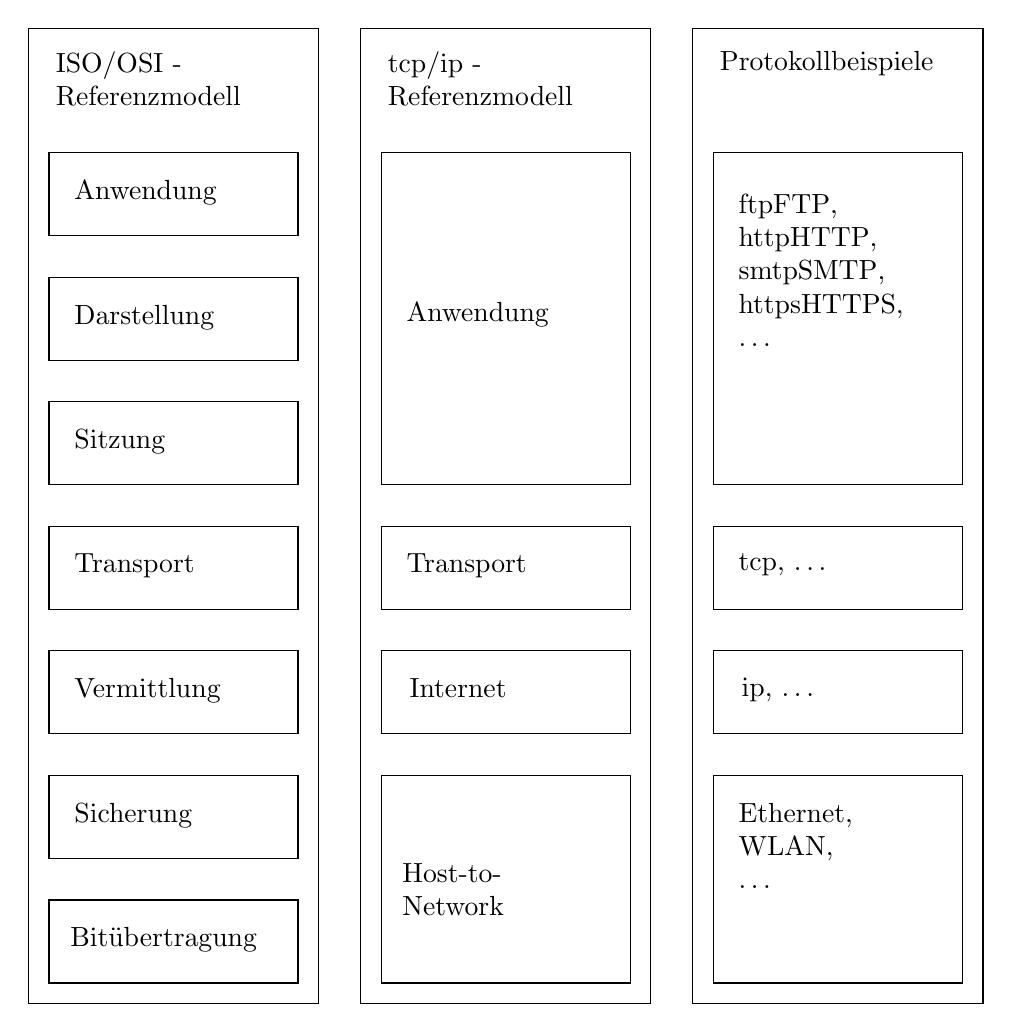
\begin{tikzpicture}[x=0.75pt,y=0.75pt,yscale=-1,xscale=1]
%uncomment if require: \path (0,501); %set diagram left start at 0, and has height of 501

%Shape: Rectangle [id:dp14661524820943694] 
	\draw   (30,80) -- (150,80) -- (150,120) -- (30,120) -- cycle ;
%Shape: Rectangle [id:dp23125445775015252] 
	\draw   (30,140) -- (150,140) -- (150,180) -- (30,180) -- cycle ;
%Shape: Rectangle [id:dp6073056454848718] 
	\draw   (30,200) -- (150,200) -- (150,240) -- (30,240) -- cycle ;
%Shape: Rectangle [id:dp23082948060985675] 
	\draw   (30,260) -- (150,260) -- (150,300) -- (30,300) -- cycle ;
%Shape: Rectangle [id:dp9194855176265426] 
	\draw   (30,320) -- (150,320) -- (150,360) -- (30,360) -- cycle ;
%Shape: Rectangle [id:dp15002411511254277] 
	\draw   (30,380) -- (150,380) -- (150,420) -- (30,420) -- cycle ;
%Shape: Rectangle [id:dp7659278004980776] 
	\draw   (30,440) -- (150,440) -- (150,480) -- (30,480) -- cycle ;
%Shape: Rectangle [id:dp9384630671201377] 
	\draw   (190,80) -- (310,80) -- (310,240) -- (190,240) -- cycle ;
%Shape: Rectangle [id:dp2886585382725697] 
	\draw   (190,260) -- (310,260) -- (310,300) -- (190,300) -- cycle ;
%Shape: Rectangle [id:dp21363285213042427] 
	\draw   (190,320) -- (310,320) -- (310,360) -- (190,360) -- cycle ;
%Shape: Rectangle [id:dp8925292617835479] 
	\draw   (190,380) -- (310,380) -- (310,480) -- (190,480) -- cycle ;
%Shape: Rectangle [id:dp3368203067527751] 
	\draw   (20,20) -- (160,20) -- (160,490) -- (20,490) -- cycle ;
%Shape: Rectangle [id:dp15663893324336597] 
	\draw   (180,20) -- (320,20) -- (320,490) -- (180,490) -- cycle ;
%Shape: Rectangle [id:dp8662901688968356] 
	\draw   (350,80) -- (470,80) -- (470,240) -- (350,240) -- cycle ;
%Shape: Rectangle [id:dp3591838539345735] 
	\draw   (350,260) -- (470,260) -- (470,300) -- (350,300) -- cycle ;
%Shape: Rectangle [id:dp5202028765817157] 
	\draw   (350,320) -- (470,320) -- (470,360) -- (350,360) -- cycle ;
%Shape: Rectangle [id:dp2946006756790316] 
	\draw   (350,380) -- (470,380) -- (470,480) -- (350,480) -- cycle ;
%Shape: Rectangle [id:dp48123403892662564] 
	\draw   (340,20) -- (480,20) -- (480,490) -- (340,490) -- cycle ;

% Text Node
	\draw (41,92) node [anchor=north west][inner sep=0.75pt]   [align=left] {Anwendung};
% Text Node
	\draw (41,152) node [anchor=north west][inner sep=0.75pt]   [align=left] {Darstellung};
% Text Node
	\draw (41,212) node [anchor=north west][inner sep=0.75pt]   [align=left] {Sitzung};
% Text Node
	\draw (41,272) node [anchor=north west][inner sep=0.75pt]   [align=left] {Transport};
% Text Node
	\draw (41,332) node [anchor=north west][inner sep=0.75pt]   [align=left] {Vermittlung};
% Text Node
	\draw (41,392) node [anchor=north west][inner sep=0.75pt]   [align=left] {Sicherung};
% Text Node
	\draw (39,452) node [anchor=north west][inner sep=0.75pt]   [align=left] {Bitübertragung};
% Text Node
	\draw (201,272) node [anchor=north west][inner sep=0.75pt]   [align=left] {Transport};
% Text Node
	\draw (202.49,332) node [anchor=north west][inner sep=0.75pt]   [align=left] {Internet};
% Text Node
	\draw (199,421) node [anchor=north west][inner sep=0.75pt]   [align=left] {Host-to-\\Network};
% Text Node
	\draw (201,151) node [anchor=north west][inner sep=0.75pt]   [align=left] {Anwendung};
% Text Node
	\draw (32,30) node [anchor=north west][inner sep=0.75pt]   [align=left] {ISO/OSI - \\Referenzmodell};
% Text Node
	\draw (192,30) node [anchor=north west][inner sep=0.75pt]   [align=left] {\gls{tcp}/\gls{ip} - \\Referenzmodell};
% Text Node
	\draw (361,272) node [anchor=north west][inner sep=0.75pt]   [align=left] {\gls{tcp}, \ldots};
% Text Node
	\draw (362.49,332) node [anchor=north west][inner sep=0.75pt]   [align=left] {\gls{ip}, \ldots};
% Text Node
	\draw (361,392) node [anchor=north west][inner sep=0.75pt]   [align=left] {Ethernet, \\WLAN,\\\ldots};
% Text Node
	\draw (361,92) node [anchor=north west][inner sep=0.75pt]   [align=left] {\\\glslink{ftp}{FTP},\\\glslink{http}{HTTP},\\\glslink{smtp}{SMTP},\\\glslink{https}{HTTPS}, \\\ldots};
% Text Node
	\draw (352,30) node [anchor=north west][inner sep=0.75pt]   [align=left] {Protokollbeispiele};


\end{tikzpicture}

		}
	\end{figure}

	\begin{figure}[htp]
		\centering
		\caption{Vergleich der Requestzeiten\label{fig:timeOfRequests}}
		\pgfplotsset{width=\textwidth}
		\resizebox{\textwidth}{!}{
			\pgfplotstableread{include/tikzDiagrams/time.dat}{\table}

\begin{tikzpicture}

    \begin{axis}[
        xmin = 1, xmax = 10,
        ymin = 0, ymax = 80,
        grid = both,
        minor tick num = 1,
        major grid style = {lightgray},
        minor grid style = {lightgray!25},
        width = \textwidth,
        legend cell align = {left},
        legend pos = north east,
        xlabel = {Nummer der Anfrage},
        ylabel = {Zeit in Millisekunden}
    ]
        \addplot[blue, smooth, ultra thick] table [x ={x}, y = {y1}] {\table};

        \addplot[red, smooth, ultra thick] table [x ={x}, y = {y2}] {\table};

        \addplot[green, smooth, ultra thick] table [x = {x}, y = {y3}] {\table};

        \legend{
            Direkte~\gls{sql}-Abfrage,
            \glslink{autorisierung}{Autorisierte}~\gls{api}-Anfrage,
            \glslink{autorisierung}{Unautorisierte}~\gls{api}-Anfrage
        }

    \end{axis}
\end{tikzpicture}
		}
	\end{figure}

	\begin{figure}[htp]
		\centering
		\caption{Sequenzdiagramm einer Anfrage\label{fig:appsequence}}
		\pgfplotsset{width=\textwidth}
		\fbox{
			\begin{sequencediagram}

	\newthread{client}{:Client}
	\newinst[1]{oauth}{:\nameref{subsec:autorisierungsserver}}
	\newinst[1]{webservice}{:\nameref{subsec:webservice}}
	\newinst[1]{lfid}{:\lfidSystem}

	\begin{sdblock}{\nameref{subsec:oauth-2.0}}{}
		\begin{call}
		{client}
		{\shortstack{\gls{jwt}\\beantragen}}
		{oauth}
		{\shortstack{\gls{jwt}\\schicken}}
			\postlevel
		\end{call}
	\end{sdblock}

	\begin{sdblock}{\gls{http} Anfrage}{}
		\begin{call}
		{client}
		{\shortstack{Daten\\zusammen mit\\\gls{jwt} beantragen}}
		{webservice}
		{Daten zurückschicken}
			\begin{sdblock}{\nameref{subsec:oauth-2.0}}{}
				\begin{call}
				{webservice}
				{\gls{jwt} validieren}
				{oauth}
				{Rechte bestätigen}
					\postlevel
				\end{call}
			\end{sdblock}
			\begin{sdblock}{\gls{sql}}{}
				\begin{call}
				{webservice}
				{\shortstack{\gls{sql}-Anfrage\\abschicken}}
				{lfid}
				{\shortstack{Angefragte Daten\\zurückschicken}}
					\postlevel
				\end{call}
			\end{sdblock}
			\postlevel
		\end{call}
	\end{sdblock}

\end{sequencediagram}
		}
	\end{figure}

	\begin{figure}[htp]
		\centering
		\caption{Pseudodiagramm der relevanten Datenbanktabellen \label{fig:lfiddatabase}}
		\pgfplotsset{width=\textwidth}
		\fbox{
			\begin{tikzpicture}
	\pic {entity={ssa}{~~~sids\_stars\_approache~~~}{
		custareaCode \\
		countryCode \\
		icaoCode \\
		portIdent \\
		sidStarApproachIdent \\
		sidStarApproacheTyp \\
		routeTyp \\
		transitionIdent \\
		sequenceNumber
	}};
	\pic[right=of ssa] {entity={country}{country}{
		countryCode \\
		custareaCode \\
		icaoCode \\
		countryName \\
		displayFilter
	}};
	\pic[below=of country] {entity={airport}{airport}{
		custareaCode \\
		countryCode \\
		icaoCode \\
		ident
	}};
	\pic[below=of airport] {entity={waypoint}{waypoint}{
		custareaCode \\
		countryCode \\
		regnArptCode \\
		regnArptIcaoCode \\
		ident \\
		icaoCode
	}};
	\pic[below=of ssa] {entity={navaid}{navaid}{
		custareaCode \\
		countryCode \\
		icaoCode \\
		arptIdent \\
		arptIcaoCode \\
		ident \\
		typ \\
		classField1 \\
		classField2
	}};
	\node[draw, shape=rectangle, below=of waypoint, text width=0.5\textwidth]
	{Bemerkung: Zur besseren Übersichtlichkeit sind hier nur die Attribute dargestellt, welche als Primärschlüssel gekennzeichnet sind.};
\end{tikzpicture}

		}
	\end{figure}

	\begin{figure}[htp]
		\centering
		\caption{HTTP-Methoden S. 1\label{fig:http-methoden-S1}}
		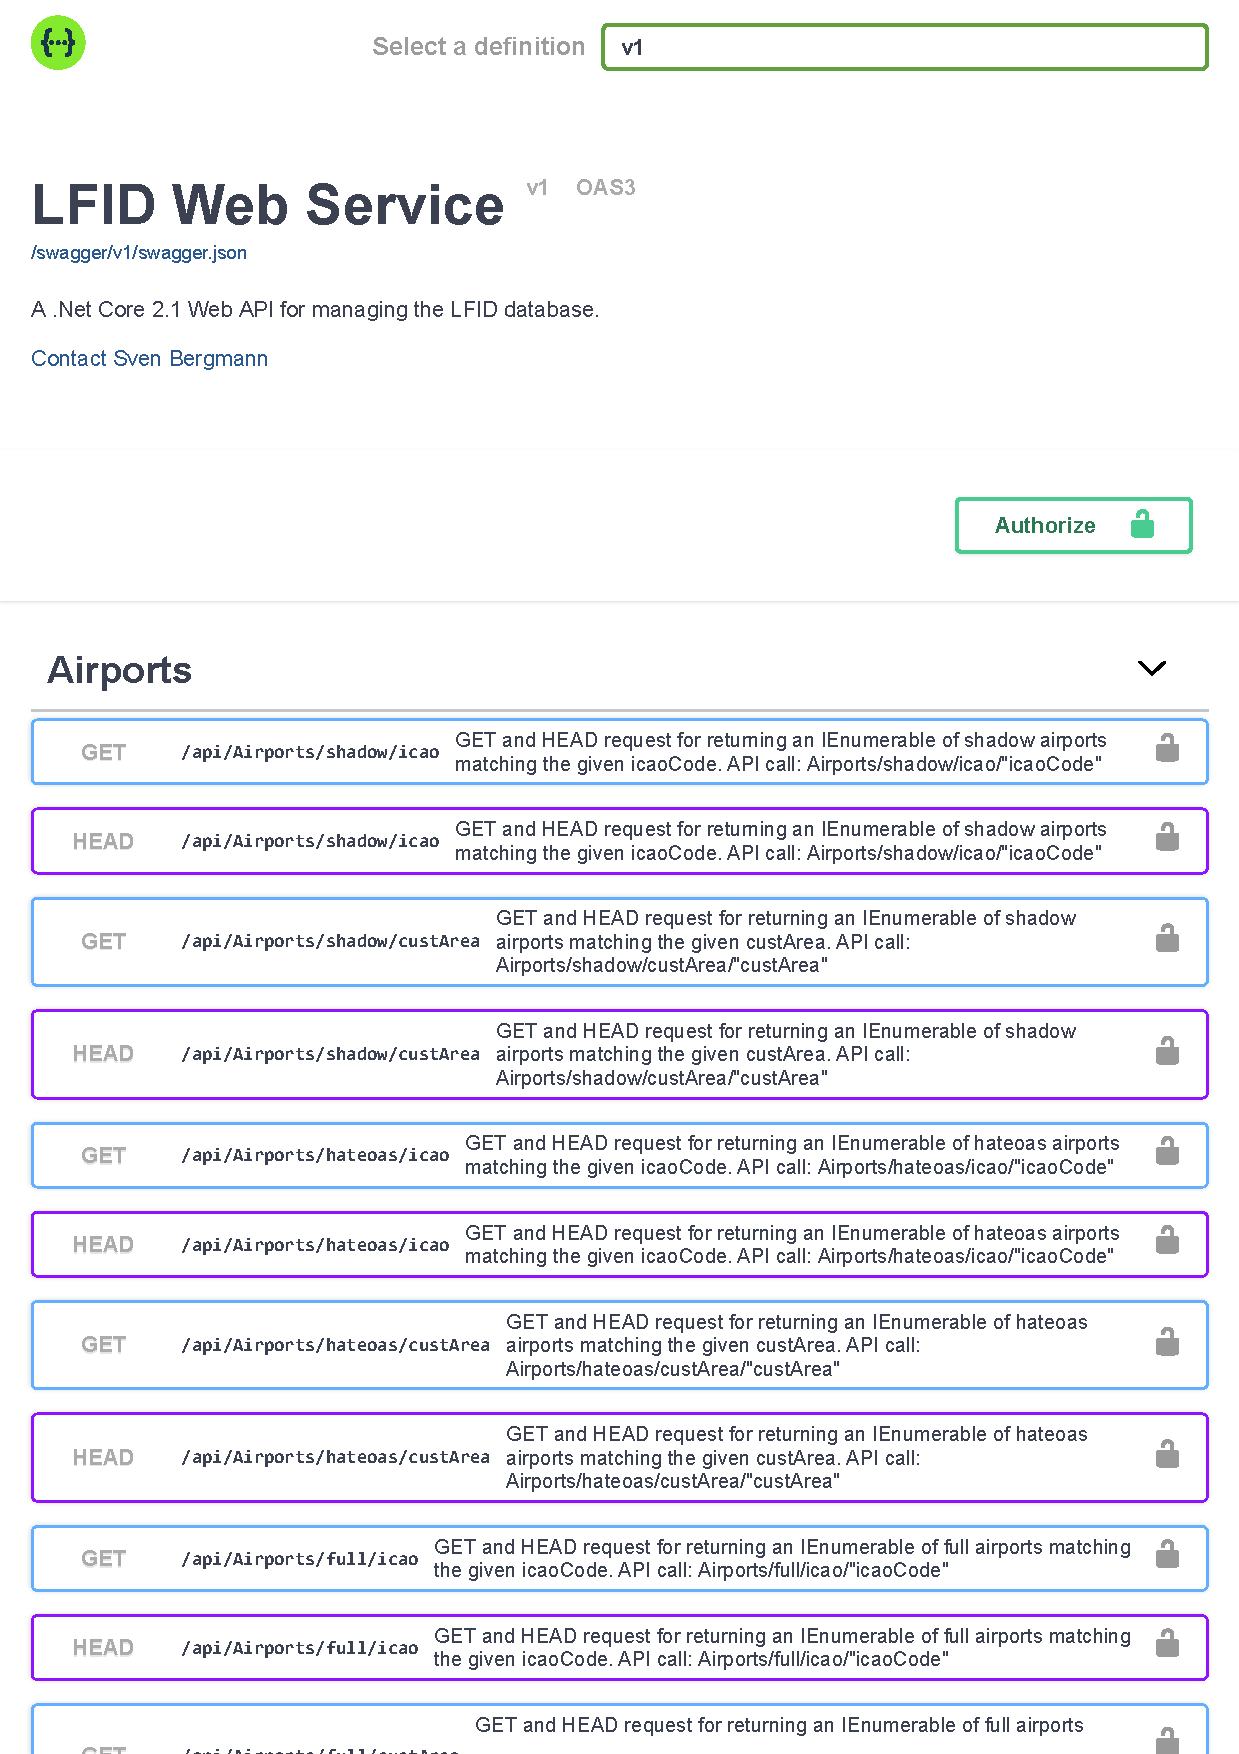
\includegraphics[page=1,width=.9\textwidth]{include/img/SwaggerUI}
	\end{figure}

	\begin{figure}[htp]
		\centering
		\caption{HTTP-Methoden S. 2\label{fig:http-methoden-S2}}
		\includegraphics[page=2,width=.9\textwidth]{include/img/SwaggerUI}
	\end{figure}

	\begin{figure}[htp]
		\centering
		\caption{HTTP-Methoden S. 3\label{fig:http-methoden-S3}}
		\includegraphics[page=3,width=.9\textwidth]{include/img/SwaggerUI}
	\end{figure}